\section{Distributed Counting for Elephant Flow}\label{sec:to}
\subsection{Elephant Flow Counting Problem}\label{sec:to-prob}
We use a simple example to explain why counting elephant flows could be a problem.
Considering a simple network shown in Fig.~\ref{fig:exam-topo5}, where 5 switches $S_1$--$S_5$ are linearly connected.
We assume there are 20 flows in this network, 4 of which are the elephant flows with 4 bytes at most, and the rest are the mice flows with only 1 byte, following the 80/20 rule.
We also assume a simple placement of the counting tasks: each switch counts 4 flows.
Next, we specifically consider the following two distributions of the elephant flows.
The first distribution evenly places the elephant flows, \eg, 4 of the 5 switches count 1 elephant flow respectively, namely ``average case'', while the second distribution assumes the 4 elephant flows are gathered in a single switch, namely ``dominant case''.
Based on the above typical cases, we analyze the memory usage of different counting approaches.

\begin{figure}[t]
    \centering
    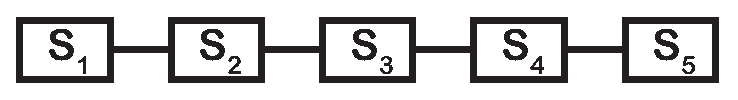
\includegraphics[width=0.6\linewidth]{pic/exam-topo5}
    \caption{Example topology.
    }
    \label{fig:exam-topo5}
    \vspace{-0.1in}
\end{figure}

\begin{figure}[t]
    \centering
    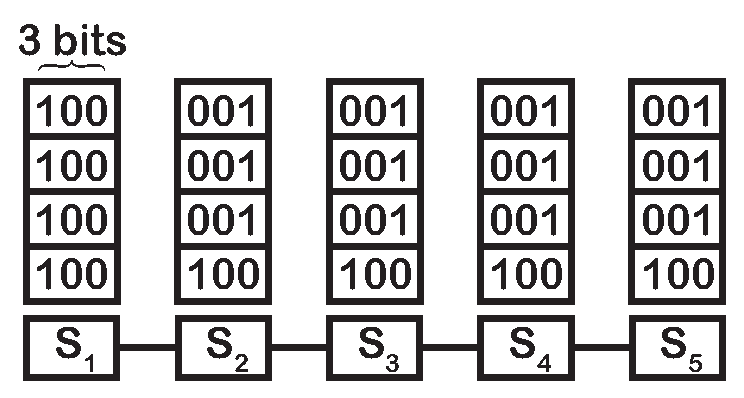
\includegraphics[width=0.6\linewidth]{pic/exam-fixed-width}
    \caption{Example of the counter arrays for the traditional large fixed-width counter solution.
    }
    \label{fig:exam-fixed-width}
    \vspace{-0.1in}
\end{figure}

The fixed-width approach always assumes the worst case, \ie, each switch will allocate 4 counters for elephant flows, no matter in average or dominant case.
As a result, it takes 60 bits in total, since a 4-byte elephant flow takes 3 bits for counting, as shown in Fig.~\ref{fig:exam-fixed-width}.
BRICK can largely save the memory in the average case, because it can flexibly extend the 1-bit bucket.
As shown in Fig.~\ref{fig:exam-brick-avg}, it consumes 30 bits in total to handle all possible average cases.
However, in dominant cases, BRICK also has to allocate 12 bits for each switch, since it cannot predict which switch will be the hot spot, as shown in Fig.~\ref{fig:exam-brick-dmn}.
In other words, in this simple example, BRICK will consume the same memory with the fixed-width approach, if it wants to avoid exceeding the switch memory in any possible case.

We note that in practice, we have bare knowledge of the flow numbers and sizes.
This fact will benefit the actual performance of BRICK, since it can adaptively extend the counter.
However, the above analysis also shows that BRICK may still fail the counting if too many elephant flows are counted in a single switch.

\begin{figure}[t]
    \centering
    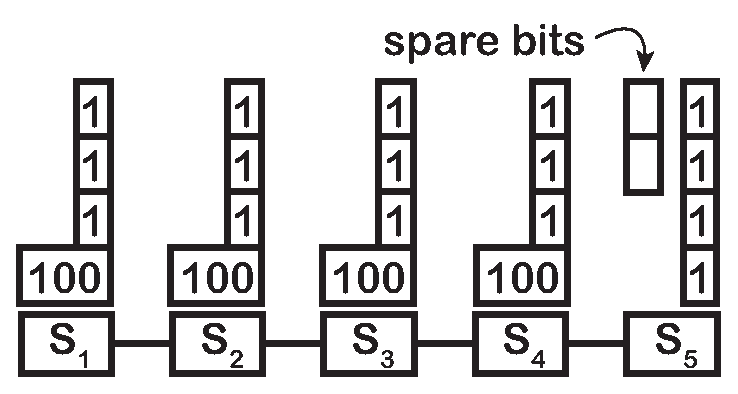
\includegraphics[width=0.6\linewidth]{pic/exam-brick-avg}
    \caption{Example of the average case of the counters for BRICK.
     }
    \label{fig:exam-brick-avg}
\end{figure}

\begin{figure}[t]
    \centering
    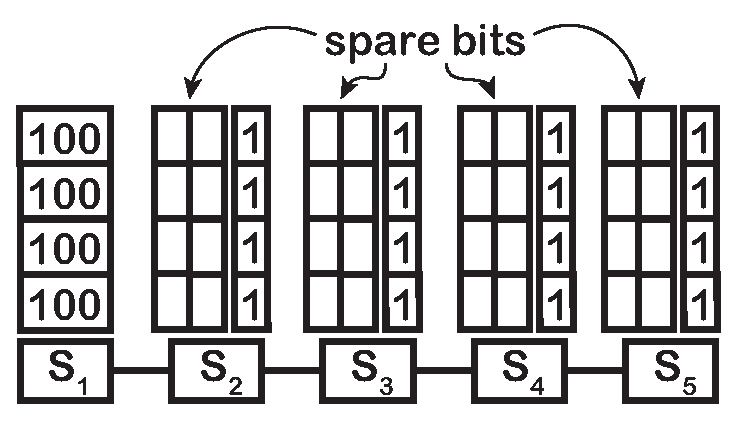
\includegraphics[width=0.6\linewidth]{pic/exam-brick-dmn}
    \caption{Example of the dominant case for BRICK.
     }
    \label{fig:exam-brick-dmn}
\end{figure}

\subsection{Basic Idea of DIAL}\label{sec:to-idea}
We propose DIAL based on a simple observation:
recall the worst case of BRICK shown in Fig.~\ref{fig:exam-brick-dmn}, when the gathered elephant flows impact the memory in a single switch, much memory remains unused in others.
Therefore, our basic idea is to exploit the spared memory in other switches as a supplement to the local memory, so that the elephant flows can be jointly counted by multiple switches instead of a single one.
Still considering the aforementioned example, we use $f_1$--$f_{20}$ to denote the 20 flows in the network, where $f_1$--$f_4$ are the 4-byte elephant flows.
DIAL allocates a set of 1-bit counters for each switch, and when a specific counter is exceeded, DIAL will use a spared counter in other switches to continue counting the flow.
Fig.~\ref{fig:exam-dial-dmn8} depicts one of the dominant cases, where all elephant flows are originally counted in the first switch.
It can be seen that 8 bits for each switch are sufficient.
For this worst case, the total memory cost is 40 bits, which is lower than that of the fixed-width approach and BRICK.
Plus, DIAL in the average case has a similar cost.

Though the above analysis shows the potential benefit of DIAL, we note that DIAL could bring much overhead if being simply applied.
The reason is that to implement the supplementary counters along a routing path, the original counting rule must be duplicated.
To be specific, DIAL has to duplicate all the counting rules to all the switches, in case any of them becomes an elephant flow.
This duplication makes DIAL impracticable for two reasons.
First, the number of counting rules increases with the number of switches, which largely consumes the flow entries in the flow table.
For example in Fig.~\ref{fig:exam-dial-dmn8}, the 20 flows will consume 100 flow entries.
Second, the counter memory is occupied right after the counting rules are installed.
That is, the counting memory cost will also increase with the number of switches.
For example in Fig.~\ref{fig:exam-dial-dmn8}, even assuming we have the pre-knowledge that there are only 4 elephant flows and that 8 bits for each switch are sufficient, DIAL still has to allocate 100 bits, since we don't know which four could grow to be elephant.

\begin{figure}[t]
    \centering
    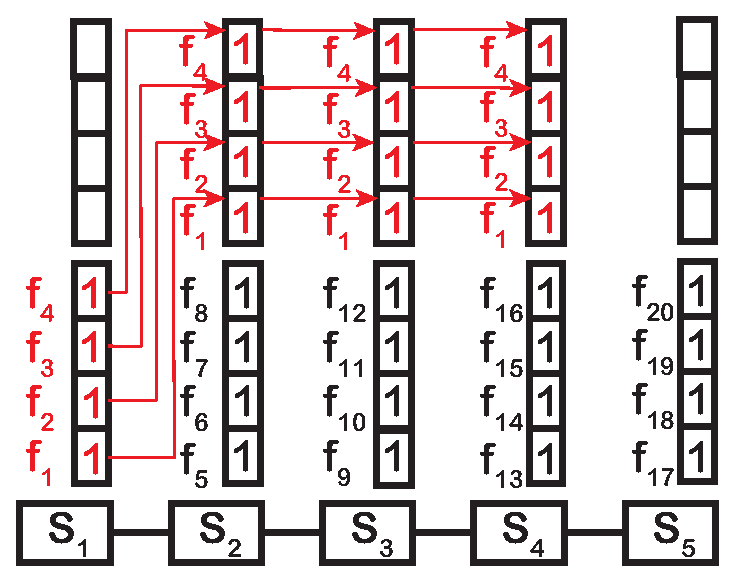
\includegraphics[width=0.6\linewidth]{pic/exam-dial-dmn8}
    \vspace{-0.1in}
    \caption{Example of the dominant case for DIAL.}
    \label{fig:exam-dial-dmn8}
    \vspace{-0.25in}
\end{figure}
